\documentclass{standalone}
\usepackage{tikz}
\usetikzlibrary{patterns, positioning}
\usepackage[sfdefault]{ClearSans} %% option 'sfdefault' activates Clear Sans as the default text font
\usepackage[T1]{fontenc}

\begin{document}
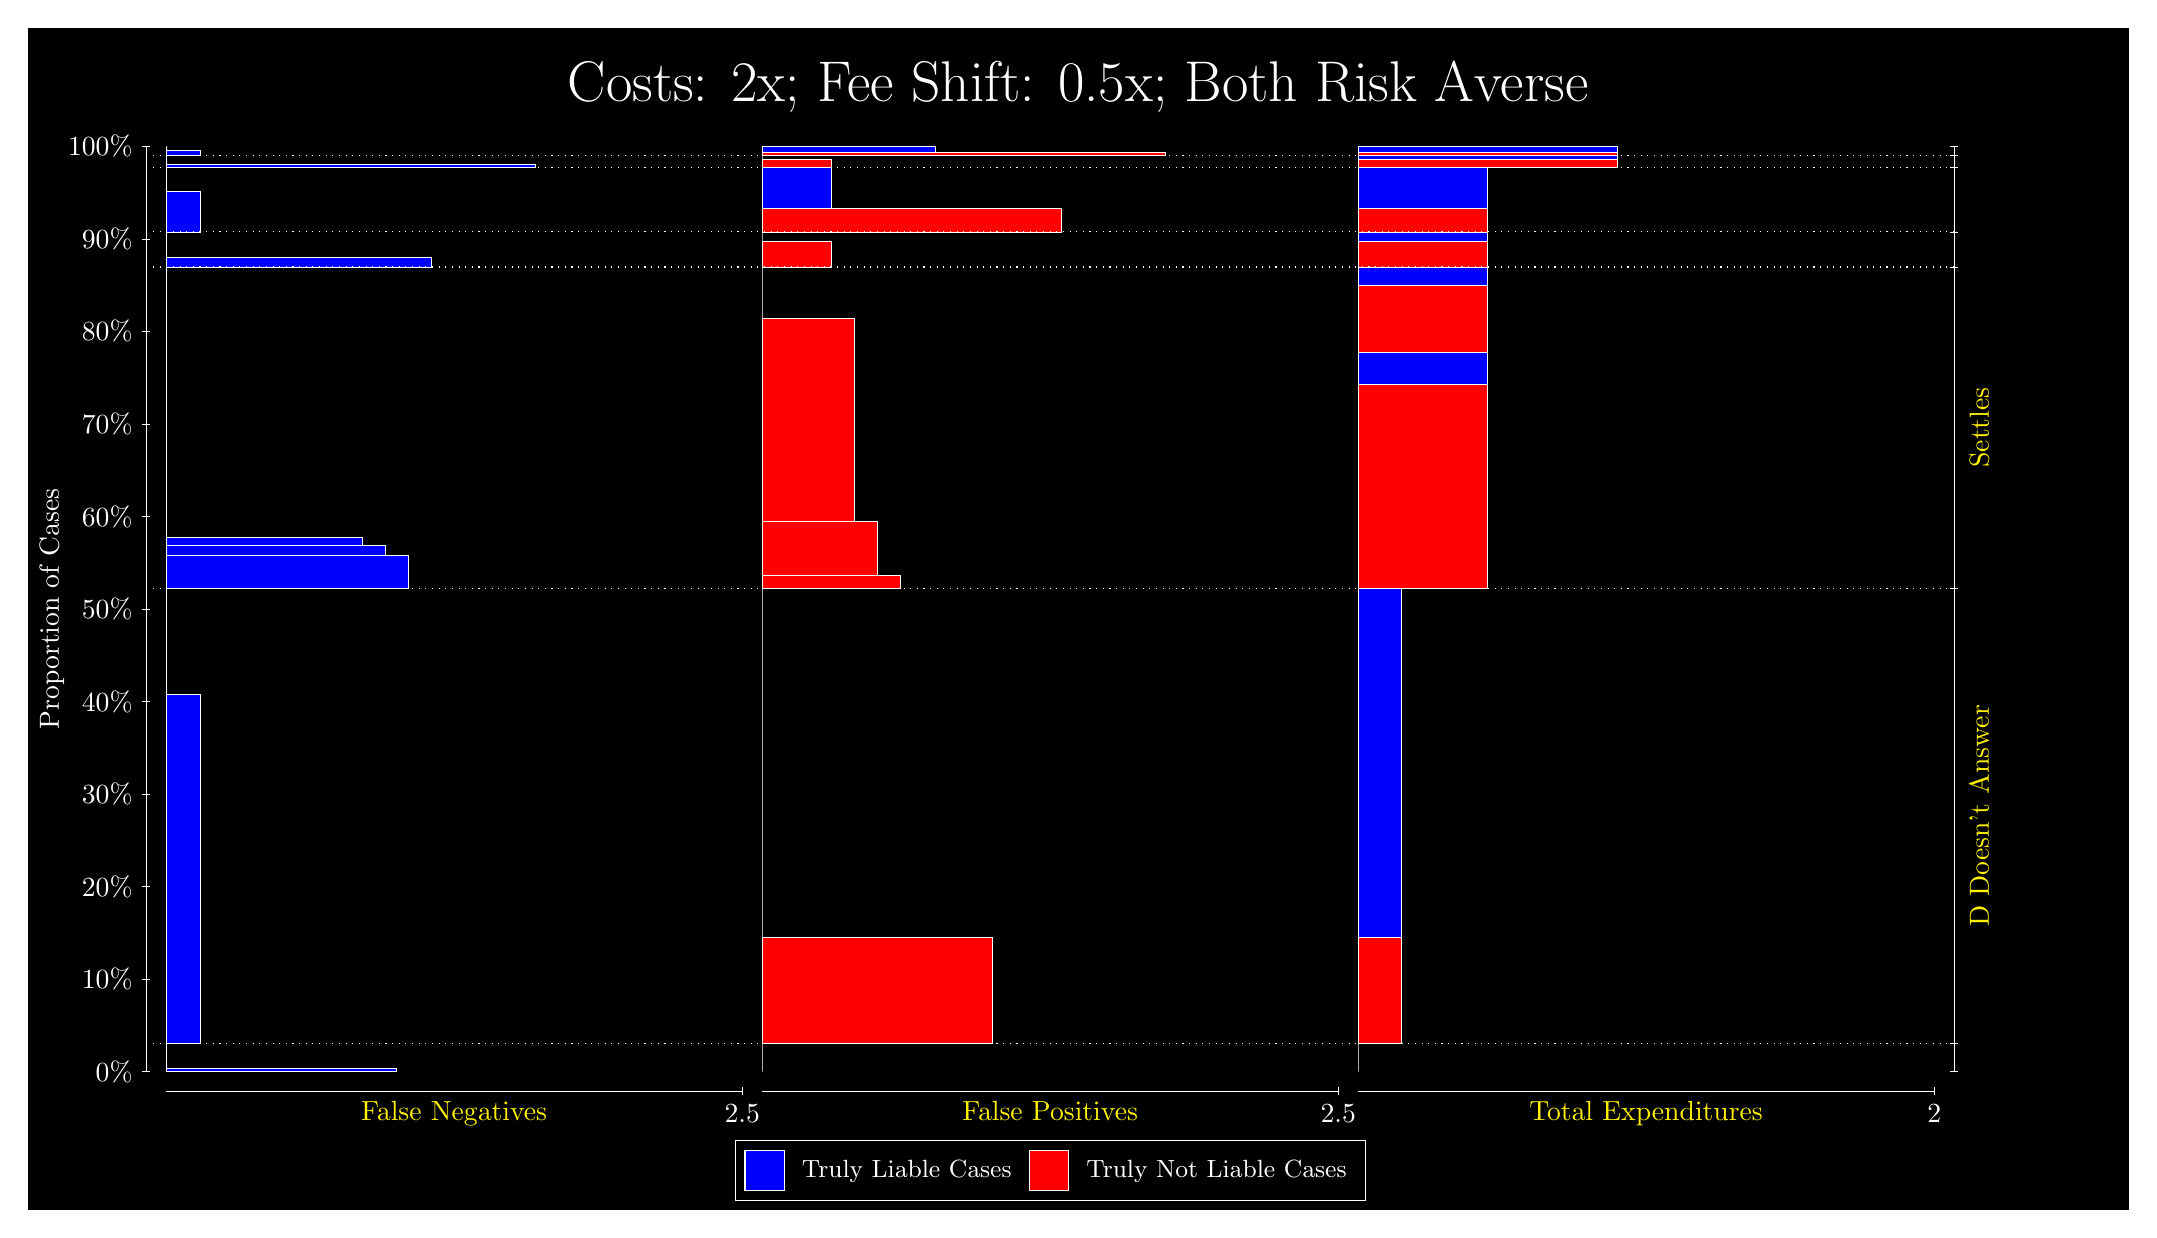
\begin{tikzpicture}
\draw[fill=black] (0,0) rectangle (26.667,15);
\draw[text=white] (0,13.5) rectangle (26.667,15) node[midway] {\huge Costs: 2x; Fee Shift: 0.5x; Both Risk Averse};
\draw[white, very thin] (1.5,1.75) -- (1.5,13.5);
\node[rotate=90, text=white, anchor=center] at (0.3, 7.625) {Proportion of Cases};
\draw[white, very thin] (1.45,1.75) -- (1.55,1.75);
\node[text=white, anchor=east] at (1.45, 1.75) {0\%};
\draw[white, very thin] (1.45,2.925) -- (1.55,2.925);
\node[text=white, anchor=east] at (1.45, 2.925) {10\%};
\draw[white, very thin] (1.45,4.1) -- (1.55,4.1);
\node[text=white, anchor=east] at (1.45, 4.1) {20\%};
\draw[white, very thin] (1.45,5.275) -- (1.55,5.275);
\node[text=white, anchor=east] at (1.45, 5.275) {30\%};
\draw[white, very thin] (1.45,6.45) -- (1.55,6.45);
\node[text=white, anchor=east] at (1.45, 6.45) {40\%};
\draw[white, very thin] (1.45,7.625) -- (1.55,7.625);
\node[text=white, anchor=east] at (1.45, 7.625) {50\%};
\draw[white, very thin] (1.45,8.8) -- (1.55,8.8);
\node[text=white, anchor=east] at (1.45, 8.8) {60\%};
\draw[white, very thin] (1.45,9.975) -- (1.55,9.975);
\node[text=white, anchor=east] at (1.45, 9.975) {70\%};
\draw[white, very thin] (1.45,11.15) -- (1.55,11.15);
\node[text=white, anchor=east] at (1.45, 11.15) {80\%};
\draw[white, very thin] (1.45,12.325) -- (1.55,12.325);
\node[text=white, anchor=east] at (1.45, 12.325) {90\%};
\draw[white, very thin] (1.45,13.5) -- (1.55,13.5);
\node[text=white, anchor=east] at (1.45, 13.5) {100\%};

\draw[white, very thin] (24.457,1.75) -- (24.457,13.5);
\draw[white, very thin] (24.407,1.75) -- (24.507,1.75);
\node[anchor=west] at (24.407, 1.75) {};
\draw[white, very thin] (24.407,2.1054) -- (24.507,2.1054);
\node[anchor=west] at (24.407, 2.1054) {};
\draw[white, very thin] (24.407,7.8893) -- (24.507,7.8893);
\node[anchor=west] at (24.407, 7.8893) {};
\draw[white, very thin] (24.407,11.967) -- (24.507,11.967);
\node[anchor=west] at (24.407, 11.967) {};
\draw[white, very thin] (24.407,12.413) -- (24.507,12.413);
\node[anchor=west] at (24.407, 12.413) {};
\draw[white, very thin] (24.407,13.228) -- (24.507,13.228);
\node[anchor=west] at (24.407, 13.228) {};
\draw[white, very thin] (24.407,13.382) -- (24.507,13.382);
\node[anchor=west] at (24.407, 13.382) {};
\draw[white, very thin] (24.407,13.5) -- (24.507,13.5);
\node[anchor=west] at (24.407, 13.5) {};

\draw[white, very thin, fill=blue] (1.75,1.75) rectangle (4.6775,1.7874);
\draw[white, very thin, fill=red] (1.75,1.7874) rectangle (1.75,2.1054);
\draw[white, very thin, fill=blue] (1.75,2.1054) rectangle (2.1891,6.5429);
\draw[white, very thin, fill=red] (1.75,6.5429) rectangle (1.75,7.8893);
\draw[white, very thin, fill=blue] (1.75,7.8893) rectangle (4.8239,8.3068);
\draw[white, very thin, fill=blue] (1.75,8.3068) rectangle (4.5312,8.438);
\draw[white, very thin, fill=blue] (1.75,8.438) rectangle (4.2384,8.5392);
\draw[white, very thin, fill=red] (1.75,8.5392) rectangle (1.75,11.967);
\draw[white, very thin, fill=blue] (1.75,11.967) rectangle (5.1167,12.087);
\draw[white, very thin, fill=red] (1.75,12.087) rectangle (1.75,12.413);
\draw[white, very thin, fill=blue] (1.75,12.413) rectangle (2.1891,12.925);
\draw[white, very thin, fill=red] (1.75,12.925) rectangle (1.75,13.228);
\draw[white, very thin, fill=blue] (1.75,13.228) rectangle (6.4341,13.273);
\draw[white, very thin, fill=red] (1.75,13.273) rectangle (1.75,13.382);
\draw[white, very thin, fill=blue] (1.75,13.382) rectangle (2.1891,13.454);
\draw[white, very thin, fill=red] (1.75,13.454) rectangle (1.75,13.5);
\draw[white, very thin, fill=red] (9.3189,1.75) rectangle (9.3189,2.0681);
\draw[white, very thin, fill=blue] (9.3189,2.0681) rectangle (9.3189,2.1054);
\draw[white, very thin, fill=red] (9.3189,2.1054) rectangle (12.246,3.4519);
\draw[white, very thin, fill=blue] (9.3189,3.4519) rectangle (9.3189,7.8893);
\draw[white, very thin, fill=red] (9.3189,7.8893) rectangle (11.075,8.0554);
\draw[white, very thin, fill=red] (9.3189,8.0554) rectangle (10.783,8.7347);
\draw[white, very thin, fill=red] (9.3189,8.7347) rectangle (10.49,11.317);
\draw[white, very thin, fill=blue] (9.3189,11.317) rectangle (9.3189,11.967);
\draw[white, very thin, fill=red] (9.3189,11.967) rectangle (10.197,12.293);
\draw[white, very thin, fill=blue] (9.3189,12.293) rectangle (9.3189,12.413);
\draw[white, very thin, fill=red] (9.3189,12.413) rectangle (13.125,12.715);
\draw[white, very thin, fill=blue] (9.3189,12.715) rectangle (10.197,13.228);
\draw[white, very thin, fill=red] (9.3189,13.228) rectangle (10.197,13.337);
\draw[white, very thin, fill=blue] (9.3189,13.337) rectangle (9.3189,13.382);
\draw[white, very thin, fill=red] (9.3189,13.382) rectangle (14.442,13.428);
\draw[white, very thin, fill=blue] (9.3189,13.428) rectangle (11.515,13.5);
\draw[white, very thin, fill=red] (16.888,1.75) rectangle (16.888,2.0681);
\draw[white, very thin, fill=blue] (16.888,2.0681) rectangle (16.888,2.1054);
\draw[white, very thin, fill=red] (16.888,2.1054) rectangle (17.437,3.4519);
\draw[white, very thin, fill=blue] (16.888,3.4519) rectangle (17.437,7.8893);
\draw[white, very thin, fill=red] (16.888,7.8893) rectangle (18.534,10.472);
\draw[white, very thin, fill=blue] (16.888,10.472) rectangle (18.534,10.889);
\draw[white, very thin, fill=red] (16.888,10.889) rectangle (18.534,11.734);
\draw[white, very thin, fill=blue] (16.888,11.734) rectangle (18.534,11.967);
\draw[white, very thin, fill=red] (16.888,11.967) rectangle (18.534,12.293);
\draw[white, very thin, fill=blue] (16.888,12.293) rectangle (18.534,12.413);
\draw[white, very thin, fill=red] (16.888,12.413) rectangle (18.534,12.715);
\draw[white, very thin, fill=blue] (16.888,12.715) rectangle (18.534,13.228);
\draw[white, very thin, fill=red] (16.888,13.228) rectangle (20.181,13.337);
\draw[white, very thin, fill=blue] (16.888,13.337) rectangle (20.181,13.382);
\draw[white, very thin, fill=red] (16.888,13.382) rectangle (20.181,13.428);
\draw[white, very thin, fill=blue] (16.888,13.428) rectangle (20.181,13.5);
\draw[white, dotted] (1.5,2.1054) -- (24.457,2.1054);
\draw[white, dotted] (1.5,7.8893) -- (24.457,7.8893);
\draw[white, dotted] (1.5,11.967) -- (24.457,11.967);
\draw[white, dotted] (1.5,12.413) -- (24.457,12.413);
\draw[white, dotted] (1.5,13.228) -- (24.457,13.228);
\draw[white, dotted] (1.5,13.382) -- (24.457,13.382);
\draw[white, very thin] (1.75,1.5) -- (9.0689,1.5);
\node[text=yellow, anchor=north] at (5.4094, 1.5) {False Negatives};
\draw[white, very thin] (9.0689,1.45) -- (9.0689,1.55);
\node[text=white, anchor=north] at (9.0689, 1.45) {2.5};

\draw[white, very thin] (9.3189,1.5) -- (16.638,1.5);
\node[text=yellow, anchor=north] at (12.978, 1.5) {False Positives};
\draw[white, very thin] (16.638,1.45) -- (16.638,1.55);
\node[text=white, anchor=north] at (16.638, 1.45) {2.5};

\draw[white, very thin] (16.888,1.5) -- (24.207,1.5);
\node[text=yellow, anchor=north] at (20.547, 1.5) {Total Expenditures};
\draw[white, very thin] (24.207,1.45) -- (24.207,1.55);
\node[text=white, anchor=north] at (24.207, 1.45) {2};


\node[text=yellow, centered, rotate=90] at (24.777, 4.9974) {D Doesn't Answer};
\node[text=yellow, centered, rotate=90] at (24.777, 9.9281) {Settles};





\draw (12.978300999999998,1.5) node[draw=none] (baseCoordinate) {};
\begin{scope}[align=center]
        \matrix[scale=0.5, draw=white, below=0.5cm of baseCoordinate, nodes={draw}, column sep=0.1cm]{
            \node[rectangle, draw, minimum width=0.5cm, minimum height=0.5cm, fill=blue] {}; &
            \node[draw=none, font=\small, text=white] (B) {Truly Liable Cases}; &
            \node[rectangle, draw, minimum width=0.5cm, minimum height=0.5cm, fill=red] {}; &
            \node[draw=none, font=\small, text=white] (B) {Truly Not Liable Cases}; \\
            };
\end{scope}

\end{tikzpicture}
\end{document}